\documentclass{minimal}
\usepackage[spanish]{babel}
\usepackage{graphicx}
\usepackage[utf8]{inputenc}
\usepackage{fancyhdr}
\usepackage{lastpage}

\pagestyle{fancy}
\fancyhf{}
\rfoot{Page \thepage\hspace{1pt} de~\pageref{LastPage}}

\title{Practica 4}
\author{Guillermo Lopez Garcia}
\begin{document}
\maketitle

\textbf{Ejercicio 3.} \\

Basicamente, a las concluciones a las que he llegado, es que de forma secuencial, la dificultad de programar es mas sencilla, pero cuando el problema adquiere un numero de elementos muy grande, se vuelve bastante ineficiente. Por otra parte, con la programacion concurrente se aprovecha mas la capacidad de multiprocesamiento, pero se satura a la cpu con demasiados hilos de ejecución vigentes con un tamaño de datos enorme.
\\
\\
A continuación, expongo los graficas generadas con gnuplot y comparacion de los 4 programas.
\\
\begin{figure}
  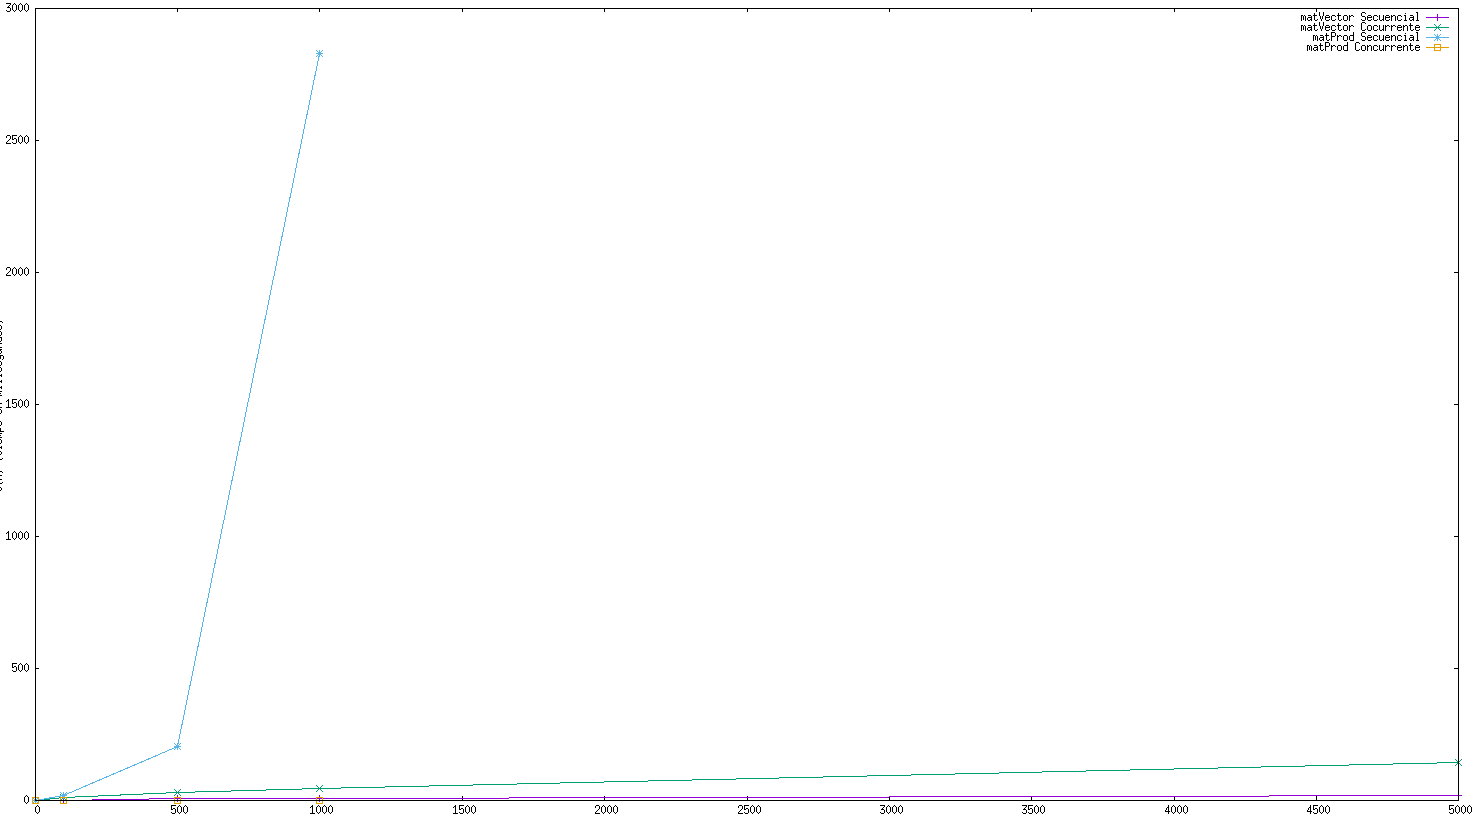
\includegraphics[width=\linewidth]{img.png}
  \caption{Compararitva de los 4 programas segun el numero de datos de entrada.}
\label{fig:comp}
\end{figure}
\\
\\
Por último solo he podido probar el funcionamiento en un sistema Linux. No tuve acceso al sistema privativo y de licencia pagada Windows.

\end{document}
